\documentclass[12pt, oneside]{report}

\usepackage[left=2.5cm, top=2.5cm, bottom=2.5cm, right=2.5cm]{geometry}

\usepackage[utf8]{inputenc}
\usepackage[T1]{polski}
\usepackage[polish]{babel}
\usepackage{hyperref}
\usepackage{physics}
\usepackage{graphicx}
\usepackage{amsthm}
\usepackage{enumitem}

\newtheorem{theorem}{Twierdzenie}
\newtheorem{lemma}{Lemat}
\newcommand\Omicron{O}

\begin{document}  
\thispagestyle{empty}
\begin{titlepage}
    \begin{center}

           \Large
    \textbf{Uniwersytet Jagielloński w Krakowie}\vspace{0.2cm}\\ Wydział Matematyki i Informatyki
               \vspace*{1cm}
               
         \vspace{3cm}
         \Large
          \textbf{Pola Kyzioł}\\\vspace{0.5cm}
         \normalsize Nr albumu: 1092406\\
             \vspace{2cm}
        \Huge
        \textbf{Algorytmy dynamiczne po dekompozycji drzewowej dla problemów grafowych o spójnych rozwiązaniach.}
      
        \vspace{1.5cm}
        \normalsize
        Praca magisterska\\
        na kierunku Informatyka Analityczna\\ \vspace{0.15cm}
        
        \vfill
        \vspace{2cm}
       \begin{minipage}{1\textwidth}
\begin{flushright}
Praca wykonana pod kierunkiem\\
dr hab. Tomasz Krawczyk\\
Instytut Informatyki Analitycznej 
\end{flushright}
\end{minipage}
        
        \vspace{2cm}
        \begin{center}
      Kraków 2019
        \end{center}
    \end{center}
\end{titlepage}

\newpage 
 \thispagestyle{empty}
\vspace{2.5cm}
\begin{flushleft}
\large \textbf{Oświadczenie autora pracy}\vspace{0.6cm}\\
\end{flushleft}

\noindent Świadom odpowiedzialności prawnej oświadczam, że niniejsza praca dyplomowa została napisana przeze mnie samodzielnie i nie zawiera treści uzyskanych w sposób niezgodny z obowiązującymi przepisami.\\

\noindent Oświadczam również, że przedstawiona praca nie była wcześniej przedmiotem procedur związanych z uzyskaniem tytułu zawodowego w wyższej uczelni.
\vspace{2cm}
\begin{center}
\begin{tabular}{lr}
................................~~~~~~~~~~~~~~~~~~~~~~~~~~~~~~~~~~~~~~&
.......................................... \\
{~~~~Kraków, dnia} & {Podpis autora pracy~~~~}
\end{tabular}
\end{center}
\vspace{5cm}
\begin{flushleft}
\large \textbf{Oświadczenie kierującego pracą}
\end{flushleft}

\noindent Potwierdzam, że niniejsza praca została przygotowana pod moim kierunkiem i~kwalifikuje się do przedstawienia jej w postępowaniu o nadanie tytułu zawodowego.
\vspace{2cm}
\begin{center}
\begin{tabular}{lr}
................................~~~~~~~~~~~~~~~~~~~~~~~~~~~~~~~~~~~~~~&
............................................ \\
{~~~~Kraków, dnia} & {Podpis kierującego pracą~~}
\end{tabular}
\end{center}
\vfill

\newpage
\tableofcontents

\newpage
  	\chapter{Dekompozycja drzewowa}
  		\section{Definicja dekompozycji i szerokości drzewowej}

Dekompozycją drzewową grafu $G$ nazywamy parę $\mathcal{T} = (T, \{X_t : t \in V(T)\})$, gdzie $T$ jest drzewem, a $\{X_t : t \in V(T)\}$
zawiera zbiory wierzchołków grafu $G$ i spełnia następujące warunki:
\begin{itemize}
	\item{Dla każdej krawędzi $\{u, v\} \in E(G)$, istnieje węzeł $t \in V(T)$, taki że $u \in X_t$ i $v \in X_t$.}
	\item{Dla każdego wierzchołka $v \in V(G)$, zbiór $\{t \in V(T): v \in X_t \}$ jest poddrzewem drzewa $T$.}
\end{itemize}
Od tej pory wierzchołki grafu wyjściowego $G$ będą nazywane po prostu \emph{wierzchołkami}, natomiast węzły drzewa $T$ będą nazywane \emph{kubełkami}.
\newline\newline
Szerokość drzewowa dekompozycji drzewowej $\mathcal{T}$ jest zdefiniowana następująco: \newline $sd_\mathcal{T} = max_{t \in V(T)} \abs{X_t - 1}$. Natomiast szerokość drzewowa grafu $G$ jest minimalną szerokością drzewową wziętą po wszystkich możliwych dekompozycjach drzewowych $G$: \newline $sd_G = min \{sd_\mathcal{T}: \mathcal{T} \text{ jest dekompozycją drzewową }G\}$.
  		
  		\section{Ładna dekompozycja drzewowa}
Dla uproszczenia posługiwania się dekompozycją drzewową przy definiowaniu algorytmów dynamicznych, będziemy używać tzw. \emph{ładnej dekompozycji drzewowej}, która została po raz pierwszy wprowadzona przez Kloks \cite{kloks}.
\newline\newline
\emph{Ładna dekompozycja drzewowa} $\mathcal{T} = (T, \{X_t\}_{t \in V(T)})$ musi spełniać następujące warunki:
\begin{itemize}
	\item{$T$ jest ukorzenione.}
	\item{Każdy \emph{kubełek} $T$ ma co najwyżej dwoje dzieci.}
	\item{Jeśli \emph{kubełek} $t$ ma dwoje dzieci $p$ i $q$, wtedy $X_t = X_p = X_q$.}
	\item{Jeśli \emph{kubełek} $t$ ma jedno dziecko $p$, to $\abs{X_t} = \abs{X_p} + 1$ \emph{oraz} $X_p \subset X_t$ albo $\abs{X_t} = \abs{X_p} - 1$ \emph{oraz} $X_t \subset X_p$.}
\end{itemize}
Ponieważ w ładnej dekompozycji drzewowej, \emph{kubełki} różnią się od siebie o co najwyżej jeden \emph{wierzchołek}, każde przejście między jednym a drugim \emph{kubełkiem} odpowiada dokładnie jednej operacji na grafie wyjściowym $G$. Każdy \emph{kubełek} ma jeden z następujących pięciu typów:
\begin{itemize}
	\item{\texttt{WPROWADZAJĄCY v} - \emph{kubełek} ten ma o jeden \emph{wierzchołek} więcej niż jego jedyne dziecko: $X_p \cup \{v\} = X_t$. Każdy wierzchołek $v \in V(G)$, ma co najmniej jeden kubełek wprowadzający.}
	\item{\texttt{ZAPOMINAJĄCY v} - \emph{kubełek} o jednym wierzchołku mniej niż jedgo jedyne dziecko: $X_t \cup \{v\} = X_p$. Jego specjalnym reprezentantem jest korzeń. Dla każdego wierzchołka $v \in V(G)$, istnieje dokładnie jeden kubełek zapominający.}
	\item{\texttt{SCALAJĄCY} - jedyny \emph{kubełek} posiadający dwoje dzieci: $X_t = X_p = X_q$, scala dwa podgrafy o przecięciu $X_t$.}
	\item{\texttt{LIŚĆ} - dla $t$ będącego liściem: $X_t = \emptyset$.}
	\item{\texttt{UZUPEŁNIAJĄCY uv} - \emph{kubełek}, który nie pojawił się w pierwotnej definicji ładnej dekompozycji drzewowej, ale ułatwia definiowanie algorytmów operujących na dekompozycjach drzewowych. \emph{Kubełek} uzupełniający wprowadza krawędź $uv \in E(G)$ (uzupełnia krawędziami reprezentację grafu $G$ w drzewie $T$). \emph{Kubełek} $t$ \texttt{UZUPEŁNIAJĄCY} $uv$ zawiera oba \emph{wierzchołki} krawędzi: $u \in X_t$ i $v \in X_t$. Dla każdego $uv$ istnieje dokładnie jeden kubełek uzupełniający i - przyjmując bez straty ogólności $t(u)$ jest przodkiem $t(v)$ (gdzie $t(v)$ to najwyższy \emph{kubełek}, taki że $v \in X_{t(v)}$) - znajduje się on pomiędzy $t(v)$ a \texttt{ZAPOMINAJĄCY v}.}
\end{itemize}

\begin{figure}
\centering
\label{kwadrat}
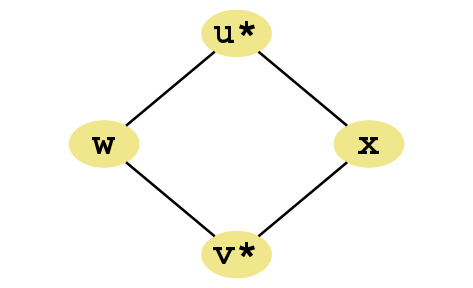
\includegraphics[width=5cm]{square_steiner_tree_standard_graph.png}
\caption{Przykładowy graf $G$.}
\end{figure}

\begin{figure}
\centering
\label{dekompozycja_kwadratu}
\makebox[\textwidth]{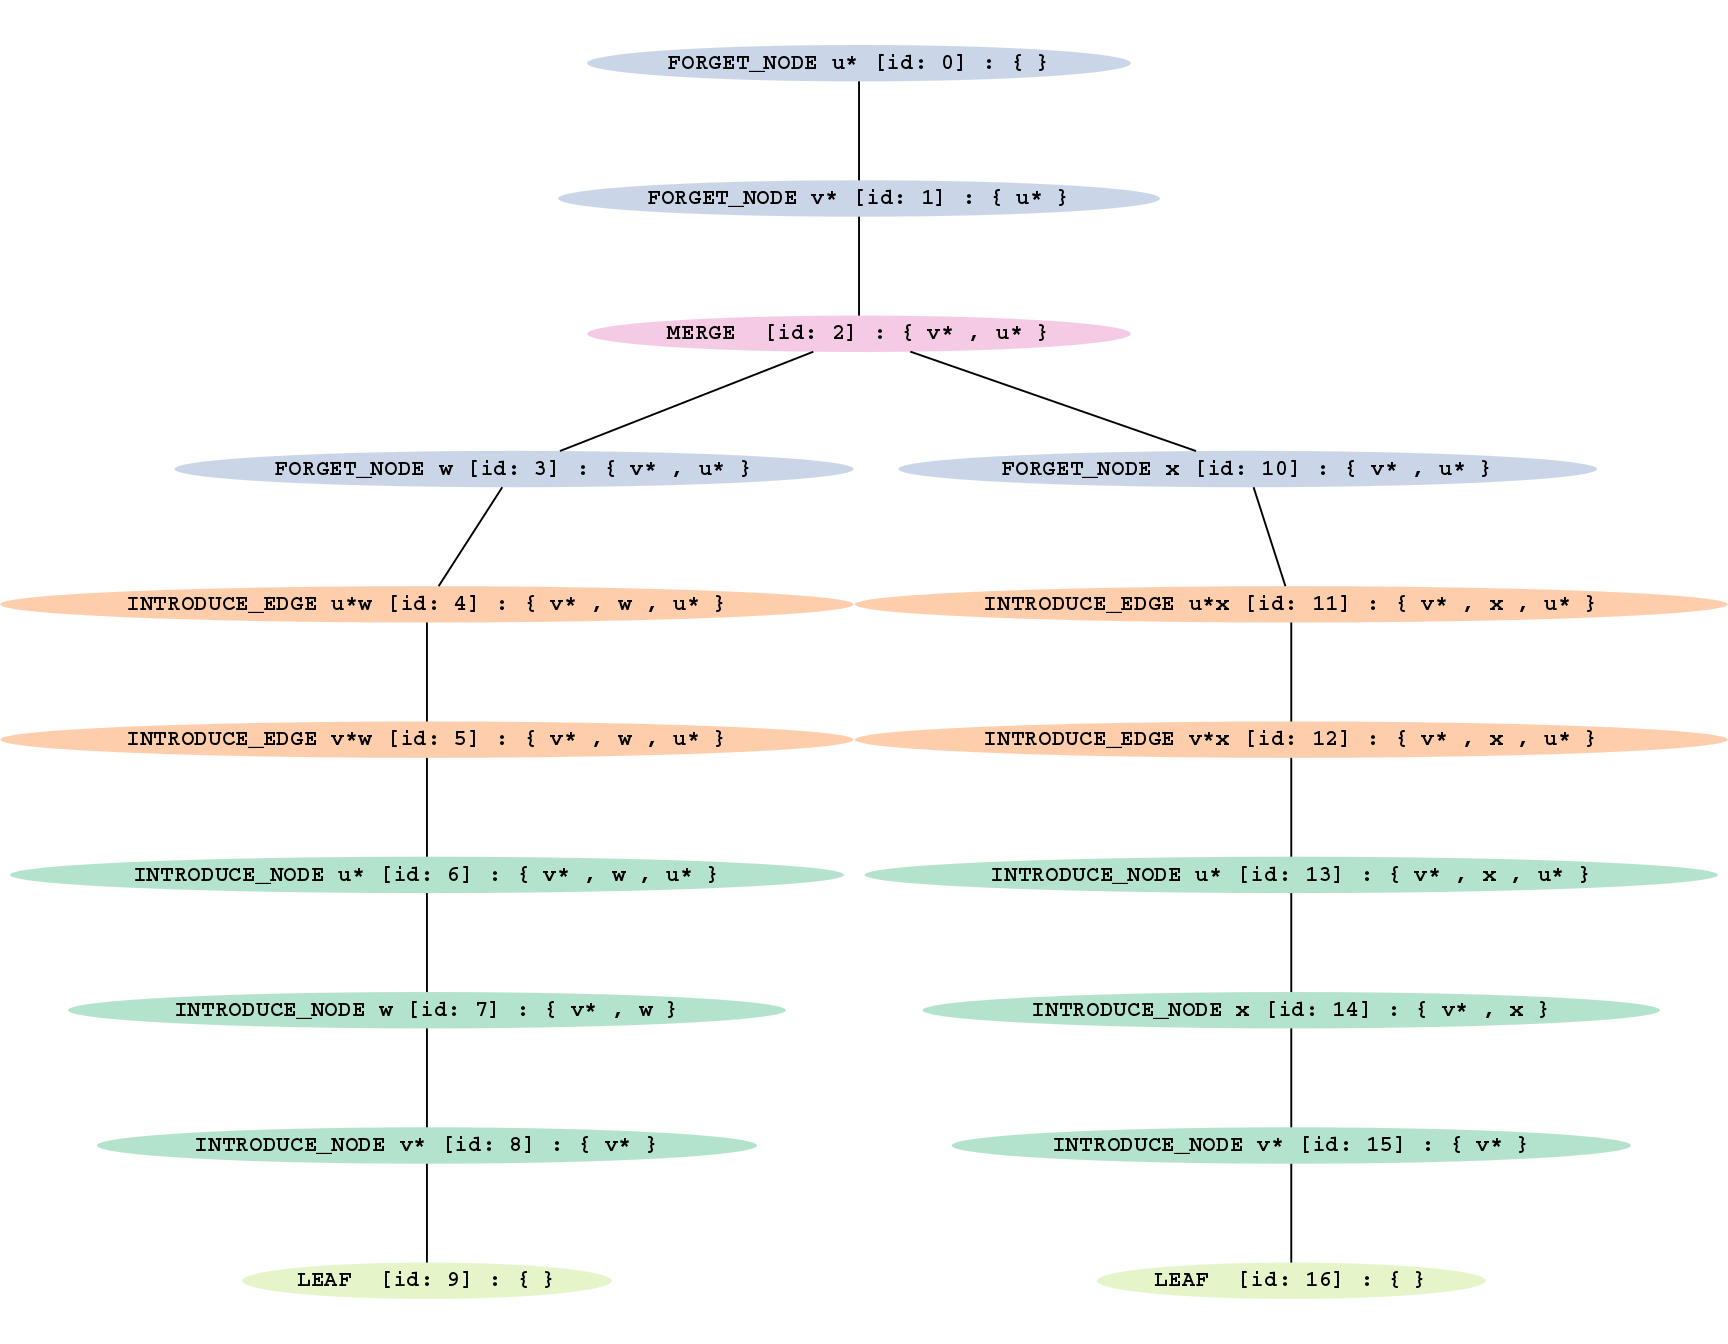
\includegraphics[width=18cm, height=14cm]{square_steiner_tree_standard.png}}
\caption{Ładna dekompozycja drzewowa grafu $G$ z rys. \ref{kwadrat}.}
\end{figure}

Na rysunku \ref{dekompozycja_kwadratu} przedstawiam ładną dekompozycję drzewową dla grafu przedstawionego na rysunku \ref{kwadrat}.

		\section{Obliczanie dekompozycji drzewowej}

Problem obliczania dekompozycji drzewowej należy do klasy problemów FPT. Odkąd Robertson i Seymour \cite{robertson&seymour} wprowadzili w latach osiemndziesiątych definicję dekompozycji drzewowej i jako pierwsi podali parametryzowany algorytm znajdowania dekompozycji drzewowej rozmiaru $\Omicron(k)$ (dla pewnej stałej $k$) o czasie działania $\Omicron(n^{f(k)})$ na grafie $n$-wierzchołkowym ($f(k)$ nigdy nie obliczyli), zostało opublikowanych wiele nowych, wielomianowych algorytmów parametryzowanych o znacznie lepszych złożonościach czasowych. Jednakże Bodlaender \cite{bodlaender} jako pierwszy podał liniowy algorytm znajdowania dekompozycji drzewowej o szerokości $k$ (o ile taka dekompozycja istnieje). 

\begin{theorem}[Bodlaender]
Dla wszystkich $k \in N$ istnieje algorytm działający w czasie liniowym, który dla danego grafu $G = (V, E)$ sprawdza, czy szerokość drzewowa tego grafu wynosi co najwyżej $k$ oraz - jeśli tak - oblicza dekompozycję drzewową $G$ o szerokości drzewowej co najwyżej $k$.  
\end{theorem}

Ponadto Kloks \cite{kloks} pokazał, że dla każdego grafu o szerokości drzewowej $k$ istnieje ładna dekompozycja drzewowa, którą można skonstruować w czasie liniowym od ilości wierzchołków grafu wyjściowego $G$.

\begin{lemma}[Kloks]
\label{kloks}
Każdy graf $G$ o szerokości drzewowej $k$ posiada ładną dekompozycję drzewową o szerokości $k$. Ponadto, jeśli $G$ jest grafem $n$-wierzchołkowym, to istnieje ładna dekompozycja drzewowa grafu $G$ o co najwyżej $4n$ kubełkach.
\end{lemma}

\begin{proof}[Dowód indukcyjny]
Graf $G$ ma szerokość drzewową $k$, wobec czego ma co najmniej $k+1$ wierzchołki. Ponadto każdy graf o szerokości drzewowej $k$ da się striangulować do postaci $k$-drzewa. Triangulacja grafu $G$ do $k$-drzewa opiera się na znalezieniu zrównoważonej dekompozycji drzewowej $\mathcal{T} = (T, \{X_t\}_{t \in V(T)})$, w której dla każdego $t \in V(T)$: $\abs{X_t} = k+1$ oraz dla każdej krawędzi $(t, p) \in E(T)$: $\abs{X_t \cap X_p} = k$, a następnie na dodaniu do $G$ krawędzi między każdą parą wierzchołków $(u, v)$, dla której istnieje kubełek nowo powstałej dekompozycji $t$ : $u \in X_t$ $\wedge$ $v \in X_t$. Algorytm równoważenia dekompozycji drzewowej został przedstawiony przez Bodlaender \cite{bodlaender} i działa on w czasie liniowym. Niech $H$ będzie striangulowanym grafem $G$ o $n$ wierzchołkach. Indukcyjnie można pokazać, że istnieje ładna dekompozycja grafu $H$ o szerokości drzewowej $k$ (w tym twierdzeniu ładna dekompozycja nie zakłada, że liście są puste).
\begin{description}
\item[Dla $n=k+1$,]{możemy wziąć trywialną dekompozycję drzewową, tj. umieścić wszystkie wierzchołki w jednym kubełku.}
\item[Dla $n>k+1$,]{$H$ posiada wierzchołek $v$, którego sąsiedzi tworzą klikę. Niech $H^{\prime}$ będzie grafem otrzymanym z $H$ poprzez usunięcie wierzchołka $v$. Z indukcji dostajemy, że istanieje ładna dekompozycja drzewowa $H^{\prime}$ o co najwyżej $4(n-1)$ kubełkach. Niech $S$ oznacza zbiór sąsiadów wierzchołka $v$. Ponieważ $S$ jest kliką (rozmiaru $k$), musi istnieć kubełek $X_t$ ładnej dekompozycji drzewowej, który zawiera $S$. Rozważmy trzy następujące przypadki dotyczące kubełka $t$:
\begin{enumerate}
\item{$t$ ma dwoje dzieci $p$ i $q$, wobec czego $X_t = X_p = X_q$. Schodzimy w dół drzewa do dowolnego z dzieci i kontynuujemy aż nie znajdziemy się w kubełku $p$ o co najwyżej jednym dziecku.}
\item{$p$ jest liściem. Jeśli $X_p = S$, tworzymy nowy kubełek $a$: $X_a = S \cup \{v\}$, który staje się dzieckiem $p$. Wpp. $X_p \neq S$, niech $z \in X_p \setminus{S}$, $p$ dostaje nowe dziecko $a$: $X_a = X_p \setminus \{z\}$. Ponieważ $S \subset X_p$ i $k = \abs{S} \leq k+1$, $X_a = S$. Dodajemy kolejny kubełek $b$ jako dziecko $a$: $X_b = S \cup {v}$.}
\label{przypadek2}
\item{$p$ ma jedno dziecko $q$. Usuwamy krawędź $(p, q)$ z drzewa. Tworzymy nowy kubełek $a$: $X_a = X_p$ i dodajemy go do drzewa jako dziecko $p$, natomiast $q$ podpinamy jako dziecko $a$. Tworzymy kolejny nowy kubełek $b$: $X_b = X_p$ i podpinamy $b$ jako dziecko $p$ (drugie dziecko). Schodzimy w dół drzewa do kubełka $b$, który jest liściem i postępujemy zgodnie z \ref{przypadek2}. Łatwo zauważyć, że wprowadzimy co najwyżej 4 nowe wierzchołki.} 
\end{enumerate}
Ponieważ dekompozycja drzewowa dla $H^{\prime}$ ma co najwyżej $4(n-1)$ wierzchołki, dekompozycja drzewowa dla $H$ ma co najwyżej $4n$ wierzchołki, co kończy dowód.}
\end{description}
\end{proof}

\begin{lemma}[Kloks]
Dla stałej $k$, mając daną dekompozycję drzewową grafu $G$ o szerokości $k$ i $\Omicron(n)$ wierzchołkach, gdzie $n$ jest liczbą wierzchołków grafu $G$, da się skonstruować ładną dekompozycję drzewową grafu $G$ o szerokości $k$ i co najwyżej $4n$ kubełkach w czasie $\Omicron(n)$. 
\end{lemma}

\begin{proof}
Dowód opiera się na konstrukcji przedstawionej w dowodzie lematu \ref{kloks}. Konstrukcja ta wymaga na wejściu striangulowanego grafu $G$ do postaci $k$-drzewa, triangulacja wymaga czasu liniowego. Szukanie odpowiedniej kolejności usuwania kubełków z $k$-drzewa $H$, czyli takiej w której sąsiedzi usuwanego kubełka indukują klikę, jest również liniowe. Dowód lematu wynika już teraz bezpośrednio z konstrukcji przedstawionej w dowodzie lematu \ref{kloks}.
\end{proof}

\newpage
  	\chapter{Klasyczne algorytmy dynamiczne}
    	\section{Drzewo Steinera}

Niniejszy algorytm został przedstawiony przez ... Mamy dany nieskierowany graf $G$ oraz zbiór wierzchołków $K$ będący podzbiorem $V(G)$, $K \subset V(G)$. Wierzchołki te nazywane są terminalami.
Naszym zadaniem jest znalezienie dla grafu $G$ takiego jego spójnego podgrafu $H$, który zawiera wszystkie terminale i jego rozmiar jest minimalny.
Zakładamy, że mamy daną ładną dekompozycję drzewową grafu wyjściowego $G$ : $\mathcal{T} = (T, \{X_t\}_{t \in V(T)})$. Dodatkowo, dla uproszczenia samego algorytmu, przyjmujemy, że każdy \emph{kubełek} zawiera przynajmniej jeden terminal. Możemy to łatwo osiągnąć - wybieramy dowolny wierzchołek ${v*}$ będący terminalem (terminale będą dla ułatwienia dodatkowo oznaczane przez *) i dodajemy go do każdego kubełka, usuwamy $\texttt{WPROWADZAJĄCY v}$ i $\texttt{ZAPOMINAJĄCY v}$, własność ładnej dekompozycji drzewowej jest zachowana z tą małą modyfikacją, że liście i korzeń nie są puste.
\newline
Zanim przejdziemy do zdefiniowania algorytmu dynamicznego dla problemu Steinera, wprowadźmy kilka dodatkowych oznaczeń.
Dla kubełka $t$, definiujemy:
\begin{description}
\item[$V_t:$]{suma wszystkich kubełków w poddrzewie ukorzenionym w $t$, włączając $X_t$, inaczej mówiąc wszystkie wierzchołki grafu wyjściowego $G$, które pojawiły się w danym poddrzewie}
\item[$E_t:$]{wszystkie krawędzie $(u, v)$, które zostały zrealizowane w poddrzewie ukorzenionym w $t$, czyli dla których istnieje kubełek $p$: $u \in X_p$ $\wedge$ $v \in X_p$} 
\item[$G_t = $]{$(V_t, E_t)$}
\end{description}

Niech $H$ będzie szukanym drzewem Steinera łączącym wszystkie terminale $K$, a $t$ jednym z kubełków $\mathcal{T}$. Przecięcie $H$ i $G_t$ tworzy las $F$, który nigdy nie jest pusty, ponieważ zawiera przynajmniej jeden wierzchołek $v*$ wprowadzony na początku do każdego kubełka. Szukane $H$ jest spójne oraz $X_t$ zawiera terminal, co implikuje, że każde drzewo należące do $F$ musi przecinać $X_t$. Ponadto każdy terminal z $K \cap V_t$ musi należeć do jednego z drzew $F$ - każdy terminal musi należeć do $F$ od momentu pojawienia się w $V_t$. Żeby utrzymać powyższe niezmienniki, trzeba w każdym kubełku rozważać wszystkie możliwe przecięcia $X_t$ z $V(F)$: $X \subset{X_t}$ oraz wszystkie partycje $X$: $\mathcal{P}$ odpowiadające drzewom (komponentom) $F$ - oznaczonym jako $C_1, \dots, C_z$ - i wybierać tylko te, które spełniają następujące warunki: 
\begin{enumerate}
\item{$K \cap V_t \subseteq V(F)$, $F$ zawiera wszystkie dotychczas wprowadzone terminale}
\item{$V(F) \cap X_t = X$, $X$ reprezentuje w danym kubełku to, co bierzemy do drzewa Steinera}
\item{dla wierzchołków należących do przecięcia $V(F) \cap X_t$, $\mathcal{P} = \{\mathcal{P}_1, \dots, \mathcal{P}_z\}$ reprezentuje dokładnie ich przynależność do poszczególnych spójnych komponentów $F$, gdzie dla każdego $y \in \{1, \dots, z\}$: $\mathcal{P}_y = V(C_y) \cap X_t$}
\end{enumerate}
Dla każdej trójki $(t, X, \mathcal{P})$ trzymamy w $c[t][X][\mathcal{P}]$ rozmiar (liczbę krawędzi) najmniejszego $F$ w $G_t$, dla którego powyższe warunki są spełnione (własność optymalnej podstruktury). Jeśli dana trójka nie spełnia wszystkich warunków $c[t][X][\mathcal{P}] = \infty$. Musimy na bieżąco śledzić partycję $\mathcal{P}$, ponieważ może się ona zmieniać wraz z każdym nowo przetwarzanym kubełkiem. Kubełki typu \texttt{SCALAJĄCY} lub \texttt{UZUPEŁNIAJĄCY uv} mogą zepsuć wcześniej poprawną partycję, tworząc cykl. Wynik końcowy odpowiada wartości $c[r][\{v*\}][\{\{v*\}\}]$, gdzie $r$ jest korzeniem. Poniżej prezentuję formuły rekurencyjne obliczania wartości $c$ ze względu na typ kubełka $t$. Dla wszystkich nie wymienionych przypadków, $c$ przyjmuje wartość $\infty$. \newline

\texttt{LIŚĆ} - każdy liść odpowiada następującemu przypadkowi:
$$c[t][\{v*\}][\{\{v*\}\}] = 0$$

\texttt{WPROWADZAJĄCY u} - w związku z tym, że $t$ jest \texttt{WPROWADZAJĄCY}, przyjmijmy następujące oznaczenia $X_t = X_{t^{\prime}} \cup u$, gdzie $t^{\prime}$ jest dzieckiem $t$. Zauważmy, że $u$ nie należał do żadnego z kubełków - przodków $t$, wobec czego krawędzie incydentne z $u$ nie zostały jeszcze wprowadzone poprzez wierzchołki \texttt{UZUPEŁNIAJĄCE} i $u$ jest wierzchołkiem izolowanym. Warunki, które muszą być spełnione:
\begin{enumerate}[label=(\roman*)]
\item $u$ jest izolowany
\item jeśli $u$ jest terminalem, musi się znaleźć w $X$
\item $u$ jako wierzchołek izolowany musi mieć swój własny, jednoelementowy komponent w $\mathcal{P}$
\end{enumerate}
Jeśli któryś z powyższych warunków nie jest spełniony, $c[t][X][\mathcal{P}] = \infty$, wpp. 
\[
c[t][X][\mathcal{P}] =  
\left \{
  \begin{tabular}{ccc}
  $c[t^{\prime}][X \setminus \{u\}][\mathcal{P} \setminus \{\{u\}\}]$ & jeśli $u \in X$,\\
  $c[t^{\prime}][X][\mathcal{P}]$ & wpp.
  \end{tabular}
\right. 
\]
\newline

\texttt{UZUPEŁNIAJĄCY uw} - iterując się po wszystkich trójkach $(t, X, \mathcal{P})$ mamy do czynienia z 3 przypadkami, które musimy rozpatrzeć osobno:

\begin{enumerate}
\item \label{notinx} $u \notin X \lor w \notin X$
\item \label{notinthesamecomponent} $u \in X \land w \in X$ oraz $u$ i $w$ są w różnych komponentach $\mathcal{P}$ ($u \in \mathcal{P}_i$, $w \in \mathcal{P}_j$, $i \neq j$)
\item \label{edgepossible} $u \in X \land w \in X$ oraz $u$ i $w$ są w tych samych komponentach $\mathcal{P}$ ($u,w \in \mathcal{P}_i$)
\end{enumerate} 
W przypadkach \ref{notinx} oraz \ref{notinthesamecomponent} krawędź $uw$ nie może należeć do rozwiązania. Natomiast w przypadku \ref{edgepossible} mamy spełnione warunki, by włączyć krawędź do rozwiązania, mamy zatem dwie możliwości - albo ją bierzemy, albo nie. Jeśli nie dorzucamy krawędzi do naszego aktualnego rozwiązania, przepisujemy częściowy wynik z $t^{\prime}$ dla tej samej partycji. W przeciwnym przypadku, nowo dodawana krawędź musiała połączyć dwa rozłączne bloki partycji $t^{\prime}$. Ponieważ optymalizujemy po rozmiarze częściowego wyniku, iterujemy się po wszystkich partycjach $\mathcal{P}^{\prime}$ kubełka $t^{\prime}$, gdzie $u$ ($\in \mathcal{P}_i$) i $w$ ($\in \mathcal{P}_j$) nie należą do tego samego komponentu ($i \neq j$), inaczej powstałby cykl, ale po połączeniu $\mathcal{P}_i$ z $\mathcal{P}_j$ dają partycję $\mathcal{P}$. Możemy to zapisać następująco:
$$c[t][X][\mathcal{P}] = \min \big\{ \min\limits_{\mathcal{P}^{\prime}} c[t^{\prime}][X][\mathcal{P}^{\prime}] + 1, \quad c[t^{\prime}][X][\mathcal{P}] \big\}$$

\texttt{ZAPOMINAJĄCY u} - niech $X_t = X_{t^{\prime}} \setminus \{u\}$. Wierzchołek $u$ może być incydentny z częściowym rozwiązaniem, wtedy trzeba popatrzeć na te partycje $\mathcal{P^{\prime}}$ kubełka $t^{\prime}$, które go zawierają, a po jego usunięciu dają nam $\mathcal{P}$. Jednakże tylko te, w których nie jest on singletonem, w przeciwnym przypadku nasze częściowe rozwiązanie nigdy nie stałoby się spójnym drzewem Steinera (wszystkie krawędzie incydentne z zapominanym wierzchołkiem są wprowadzane przed jego zapomnieniem i tylko wtedy mogą one zostać dodane do rozwiązania). Iterujemy się po wszystkich $\mathcal{P^{\prime}}$ otrzymanych z $\mathcal{P}$ poprzez dodanie $u$ do jednego z już istniejących bloków, biorąc minimum. Jednocześnie musimy pamiętać, że wierzchołek $u$ może nie należeć do końcowego rozwiązania, wtedy możemy przepisać wynik dla $t^{\prime}$, nie zmieniając parametrów. Kluczową obserwacją dla tego przypadku jest fakt, że jeśli $u$ był terminalem, nie istnieją częściowe rozwiązania dla $t^{\prime}$ nie uwzględniające $u$ (tzn. ich wynikiem jest $\infty$).
$$c[t][X][\mathcal{P}] = \min \big\{ \min\limits_{\mathcal{P}^{\prime}} c[t^{\prime}][X \cup \{u\}][\mathcal{P}^{\prime}], \quad c[t^{\prime}][X][\mathcal{P}] \big\}$$

\texttt{SCALAJĄCY} - kubełek scalający ma zawsze dwoje dzieci, dla których $X_t = X_{t_1} = X_{t_2}$. Dla tego typu kubełków musimy połączyć dwa częściowe rozwiązania - jedno pochodzące z poddrzewa $G_{t_1}$, drugie z poddrzewa $G_{t_2}$. Poniżej znajduje się klika spostrzeżeń kluczowych dla obliczania nowego częściowego rozwiązania:
\begin{enumerate}[label=(\alph*)]
\item $V_{t_1} \cap V_{t_2} = X$
\item $E_{t_1} \cap E_{t_2} = \emptyset$, ponieważ krawędzie wprowadzane są najpóźniej jak to możliwe, tj. przed kubełkami typu \texttt{ZAPOMINAJĄCY}. Zakładając nie wprost, że istnieje krawędź $uw$ zarówno w $E_{t_1}$ jak i w $E_{t_2}$, muszą również istnieć dwa kubełki - bez straty ogólności - \texttt{ZAPOMINAJĄCY u}, jeden w jednym poddrzewie, drugi w drugim poddrzewie lub naddrzewie (w zależności od tego, czy dla drugiego poddrzewa \texttt{ZAPOMINAJĄCY u} jest przodkiem \texttt{ZAPOMINAJĄCY w}). W obu przypadkach dostajemy sprzeczność, ponieważ dla każdego wierzchołka $u$ może istnieć tylko jeden \texttt{ZAPOMINAJĄCY u} (z definicji dekompozycji drzewowej).
\item Połączenie $G_{t_1}$ z $G_{t_2}$ może zawierać cykl. By uniknąć cykli autorzy algorytmu wprowadzają pomocniczą strukturę $G_{\mathcal{P}}$, która jest lasem o zbiorze wierzchołków $X$ oraz której drzewa korespondują z podziałem $\mathcal{P}$. Problem łączenia dwóch rozwiązań częściowych (dla $t_1$ oraz dla $t_2$) sprowadza się do problemu łączenia dwóch lasów $G_{\mathcal{P}_1} \cup G_{\mathcal{P}_2}$. Zauważmy, że z perspektywy wyliczania poprawnego rozwiązania dla kubełka $t$, nie jest ważne, jaki kształt mają poszczególne drzewa, istotny jest fakt, że drzewo jest grafem spójnym (między dowolną parą wierzchołków do niego należących, istnieje ścieżka).
\end{enumerate}

\begin{figure}
\centering
\label{find_n_union}
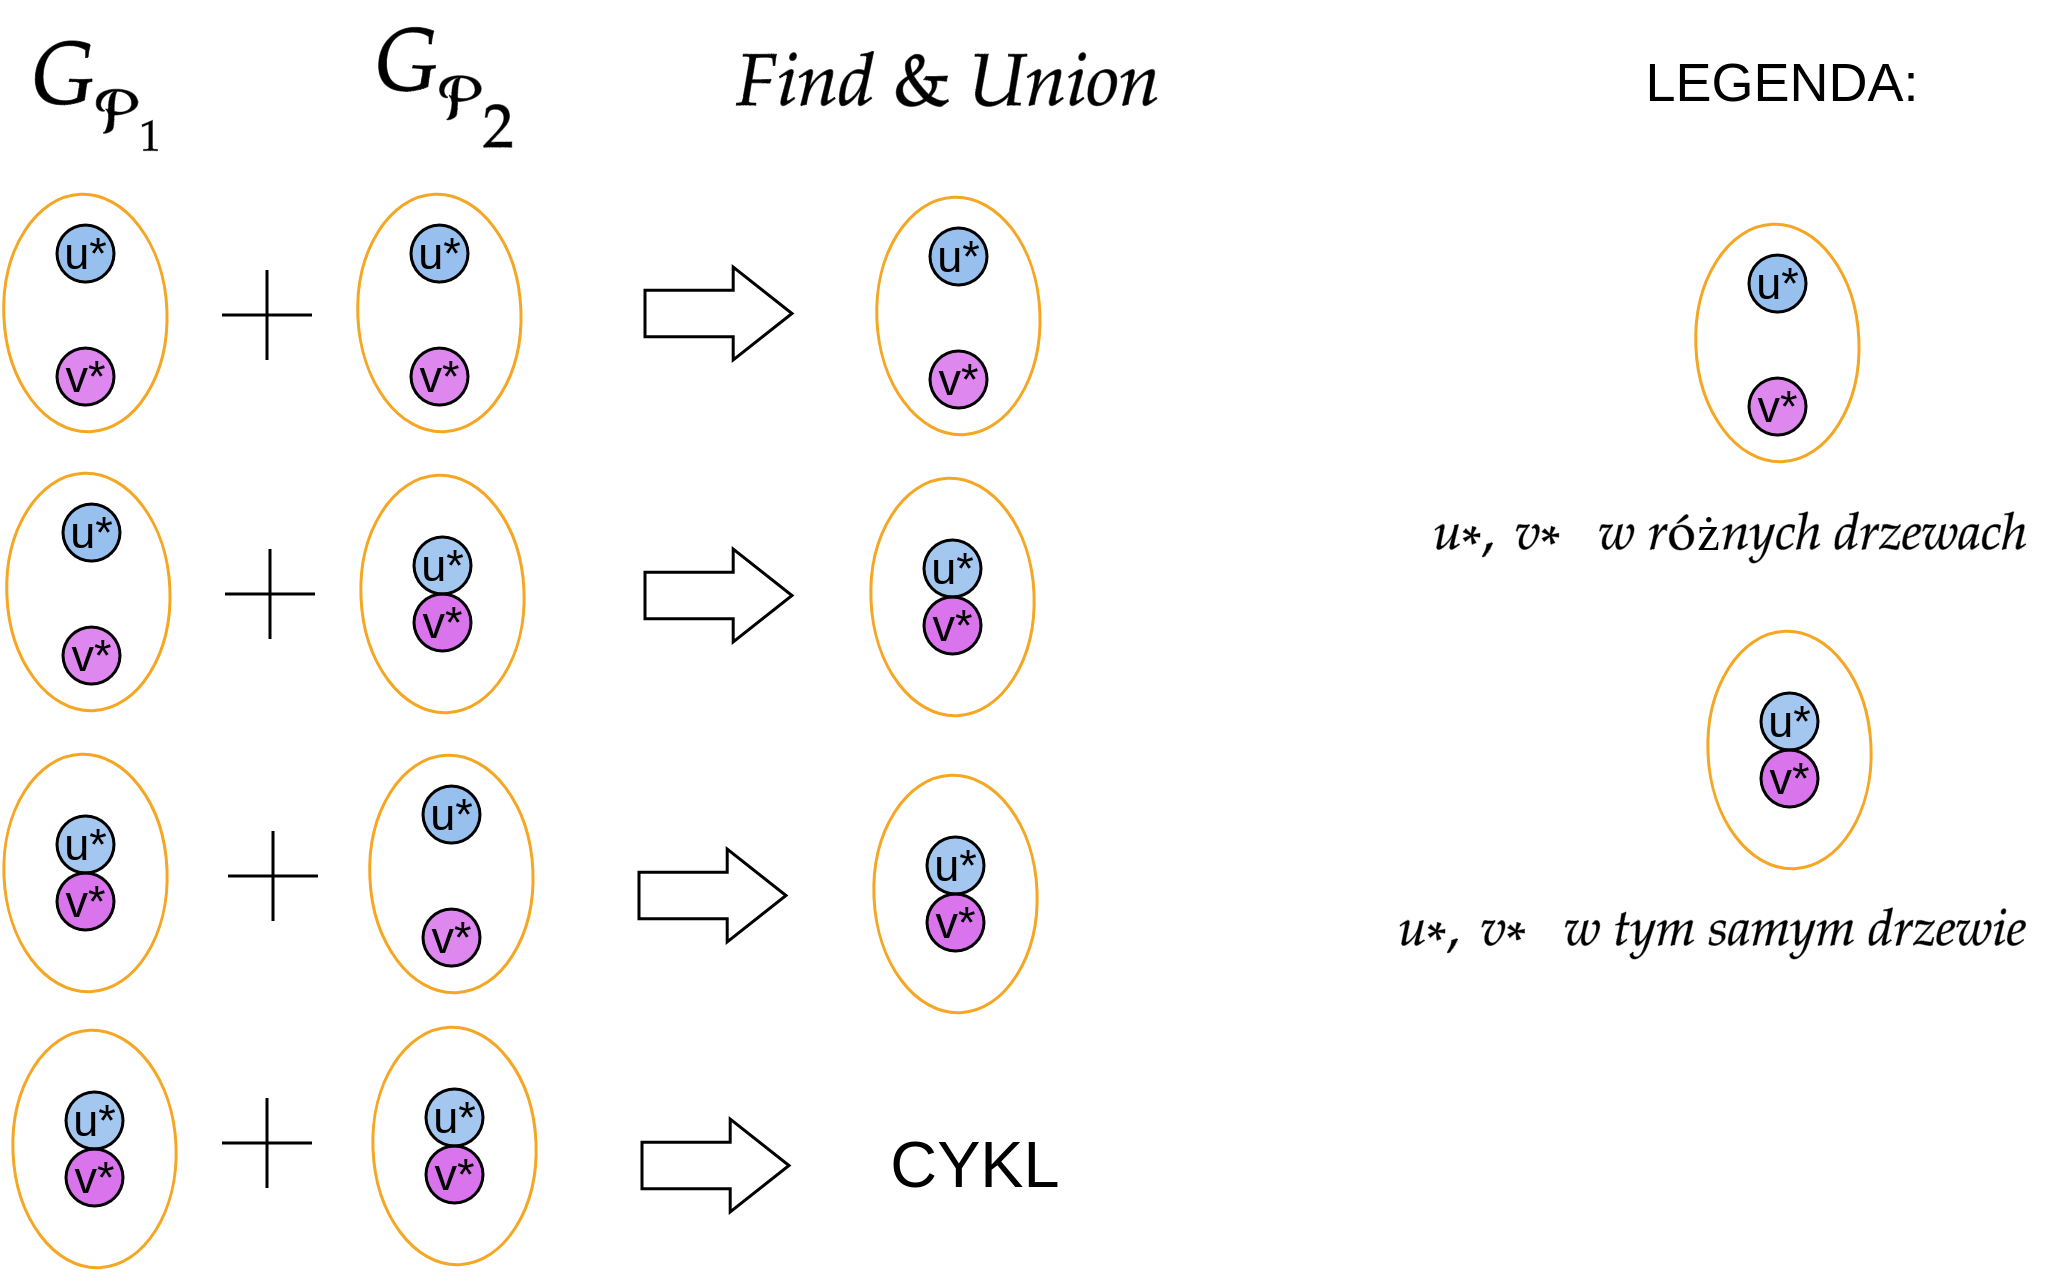
\includegraphics[width=16cm]{find_n_union7.png}
\caption{Rezultaty otrzymane w wyniku połączenia poszczególnych lasów $G_{\mathcal{P}_1}$, $G_{\mathcal{P}_2}$ w kubełku \texttt{SCALAJĄCYM} z rys. \ref{dekompozycja_kwadratu}.}
\end{figure}

Warunki, które muszą zostać spełnione przy scalaniu dwóch rozwiązań są następujące:
\begin{enumerate}[label=(\roman*)]
\item $G_{\mathcal{P}_1} \cup G_{\mathcal{P}_2}$ nie zawiera cyklu.
\item $G_{\mathcal{P}_1} \cup G_{\mathcal{P}_2}$ odpowiada $G_{\mathcal{P}}$ z dokładnością do kształtu poszczególnych drzew. 
\end{enumerate}
W implementacji powyższego algorytmu do reprezentowania problemu łączenia lasów $G_{\mathcal{P}_1}$, $G_{\mathcal{P}_2}$ wykorzystałam strukturę zbiorów rozłącznych z łączeniem według rangi i kompresją ścieżek. Dzięki niej łatwo wykryć cykl oraz zbadać, które wierzchołki są w tych samych, spójnych komponentach $\mathcal{P}$. Rysunek \ref{find_n_union} przedstawia wszystkie możliwe lasy $G_{\mathcal{P}_1}$, $G_{\mathcal{P}_2}$ dla kubełka \texttt{SCALAJĄCEGO} z rysunku \ref{dekompozycja_kwadratu} wraz z rezultatami połączenia lasów.
Końcowe rozwiązanie dla kubełka \texttt{SCALAJĄCEGO} wyliczamy na podstawie poniższego wzoru:
$$c[t][X][\mathcal{P}] = \min \limits_{\mathcal{P}_1, \mathcal{P}_2} c[t_1][X][\mathcal{P}_1] + c[t_2][X][\mathcal{P}_2]$$

Przedstawione zostały formuły rekurencyjne dla wszystkich typów kubełków. Przejdźmy zatem do wyliczenia złożoności czasowej standardowego algorytmu dynamicznego po dekompozycji drzewowej dla problemu drzewa Steinera. Poniżej znajdują się istotne spostrzeżenia:
\begin{itemize}
\item Każdy kubełek ma co najwyżek $k+2$ wierzchołki.
\item Wszystkich $X \subseteq X_t$ jest $2^{\abs{X_t}}$ a zatem nie więcej niż $2^{k+2}$.
\item Wszystkich partycji $X$ jest $\abs{X}^{\abs{X}}$ a zatem nie więcej niż $(k+2)^{k+2}$
\item Dla każdego kubełka mamy $2^{k+2} \cdot (k+2)^{k+2} = k^{\Omicron(k)}$.
\item Wartości dla każdego kubełka wyliczamy w czasie $(k^{\Omicron(k)})^2$.
\end{itemize}
 
\begin{theorem}
Mając dany $n$-wierzchołkowy graf $G$ razem ze zbiorem terminali $K \subseteq V(G)$ oraz dekompozycją drzewową o szerokości drzewowej nie większej niż $k$, można wyliczyć rozmiar minimalnego drzewa Steinera w czasie $k^{\Omicron(k)} \cdot n$. 
\end{theorem}

    	\section{Cykl Hamiltona}
    	
Mamy dany graf $G=(V, E)$. Spacer definiujemy jako naprzemienną sekwencję wierzchołków należących do $V(G)$ i krawędzi należących do $E(G)$, której początkiem i końcem są wierzchołki oraz w której każda występująca krawędź jest incydentna z wierzchołkiem poprzedzającym i następującym. Ścieżką nazywamy spacer, w którym wierzchołki się nie powtarzają. Pytamy, czy istnieje taka ścieżka $H$, która zaczyna i kończy się w tym samym wierzchołku (problem decyzyjny). Zakładamy, że mamy daną ładną dekompozycję drzewową lekko zmodyfikowanego grafu $G^{\prime}$ : $\mathcal{T} = (T, \{X_t\}_{t \in V(T)})$. Modyfikacja polega na tym, że kopiujemy wierzchołek $v$, będący w korzeniu dekompozycji drzewowej grafu $G$ (\texttt{ZAPOMINAJĄCY v}) wraz z jego krawędziami, tj. dla z każdej krawędzi $uv \in E(G)$, dostajemy dwie krawędzie $uv_1$ i $uv_2$, gdzie $v_1$ jest byłym wierzchołkiem $v$, a $v_2$ jego kopią. $\mathcal(T)$ nie zawiera kubełków \texttt{ZAPOMINAJĄCY $v_1$} oraz \texttt{ZAPOMINAJĄCY $v_2$}. Problem szukania cyklu Hamiltona modyfikujemy do problemu szukania ścieżki Hamiltona o końcach $v_1$ i $v_2$.
\newline\newline
Niech $H$ będzie szukanym cyklem Hamiltona. Przecięcie $H$ i $G_t$ składa się z wielu rozłącznych i wierzchołkowo, i krawędziowo ścieżek (również jednoelementowych, będących wierzchołkami izolowanymi), oznaczmy je jako $F$. Przecięcie to poza liśćmi nigdy nie jest puste, ponieważ wszystkie wprowadzone wierzchołki muszą należeć do częściowego rozwiązania. Szukane $H$ jest spójne, co implikuje, że każda ścieżka $C_1, \ldots, C_z$ z $F$ przecina $X_t$. Ponadto musi ona przecinać $X_t$ oboma swoimi końcami, wpp. nie dostalibyśmy spójnego rozwiązania końcowego. Biorąc pod uwagę powyższe wymagania, dostajemy że dla każdej pary ($X_t$, $F$), możemy utworzyć trzy klasy wierzchołków należących do $X_t$ (rys. \ref{hamiltonian}):
\begin{itemize}
\item wierzchołki izolowane w $F$ (o stopniu $0$)
\item wierzchołki będące końcami ścieżek $C_1, \ldots, C_z$ (o stopniu $1$)
\item wierzchołki należące do ścieżek $C_1, \ldots, C_z$ i nie będące ich końcami (o stopniu $2$)
\end{itemize}

\begin{figure}
\centering
\label{hamiltonian}
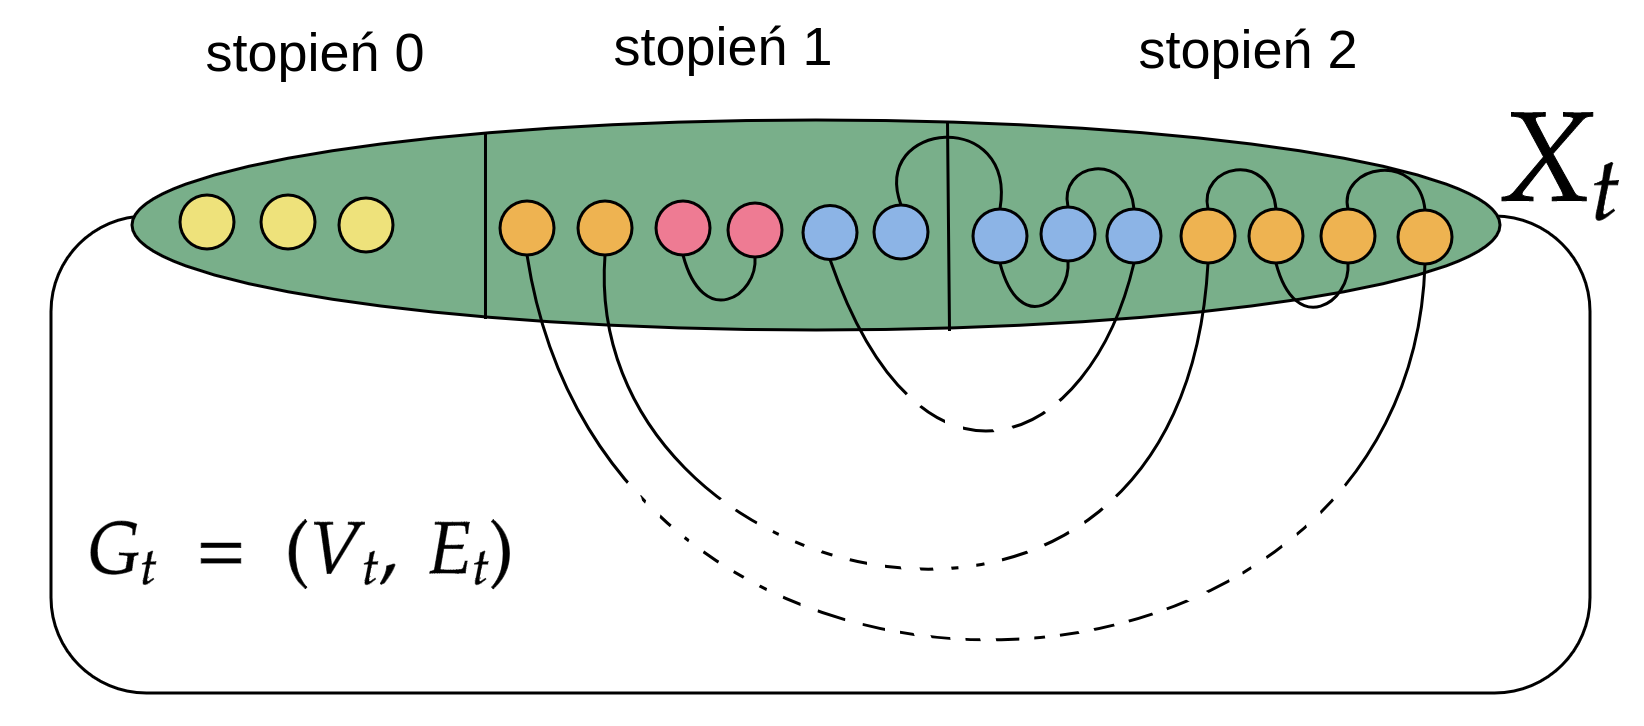
\includegraphics[width=16cm]{hamiltonian3.png}
\caption{Jedno z możliwych rozwiązań częściowych problemu znajdowania ścieżki Hamiltona dla kubełka $t$.}
\end{figure}

By utrzymać powyższe niezmienniki, w każdym kubełku $t$ musimy rozważyć wszystkie możliwe podziały zbioru $X_t$ na trzy podzbiory $\mathcal{D} = (X_{t_1}$, $X_{t_2}$, $X_{t_2})$, odpowiadające stopniom wierzchołków, które się w nich znajdują. Ponadto by w kubełkach \texttt{SCALAJĄCY} oraz \texttt{UZUPEŁNIAJĄCY uw}, nie otrzymać cyklu, musimy się przeiterować po wszystkich możliwych skojarzeniach $M$ wierzchołków ze zbioru $X_{t_1}$. Rozwiązanie częściowe jest poprawne, jeśli spełnione są następujące warunki:
\begin{enumerate}
\item $V(F) = V_t$ (wszystkie wierzchołki muszą należeć do rozwiązania)
\item $u \in X_{t_1}$ $\Leftrightarrow$ $u \in X_t$ i wierzchołek $u$ ma stopień $i$ w $F$
\item $\abs{X_{t_1}} \equiv 0 \mod 2$
\item $u$ jest skojarzone z $w$ (${u, w} \in M$) $\Leftrightarrow$ $u \in X_{t_1} \wedge w \in X_{t_1} \wedge \exists y: u \in C_y \wedge w \in C_y$ ($u$ i $w$ są końcami ścieżki $C_y$) 
\end{enumerate}  

Dla każdej trójki $(t, \mathcal{D}, M)$ trzymamy w $c[t][\mathcal{D}][M]$ $0$ lub $1$ w zależności od tego, czy powyższe warunki są spełnione. Musimy na bieżąco śledzić skojarzenie $M$, ponieważ kubełki typu \texttt{SCALAJĄCY} oraz \texttt{UZUPEŁNIAJĄCY uw} mogą utworzyć cykl. Wynik końcowy odpowiada wartości $c[r][(\emptyset, \{v_1, v_2\}, \emptyset)][\{v_1, v_2\}]$, gdzie $r$ jest korzeniem. Poniżej prezentuję formuły rekurencyjne obliczania wartości $c$ ze względu na typ kubełka $t$.
\newline\newline
\texttt{LIŚĆ} - każdy liść odpowiada następującemu przypadkowi:
$$c[t][(\emptyset, \emptyset, \emptyset)][\emptyset] = 1$$

\texttt{WPROWADZAJĄCY u} - zauważmy, że w momencie dodawania wierzchołka do $F$ jego stopień musi wynosić $0$, ponieważ żadna z incydentnych do niego krawędzi nie została jeszcze wprowadzona:

\[
c[t][(X_{t_0}, X_{t_1}, X_{t_2})][M] =  
\left \{
  \begin{tabular}{ccc}
  $c[t^{\prime}][(X_{t_0} \setminus \{u\}, X_{t_1}, X_{t_2})][M]$ & jeśli $u \in X_{t_0}$,\\
  $0$ & wpp.
  \end{tabular}
\right. 
\]

\texttt{ZAPOMINAJĄCY u} - wszystkie krawędzie incydentne do zapominanego wierzchołka zostały już wprowadzone, wobec czego zapominany wierzchołek musi mieć stopień $2$ w $F$:

$$c[t][(X_{t_0}, X_{t_1}, X_{t_2})][M] = c[t^{\prime}][(X_{t_0}, X_{t_1}, X_{t_2} \cup \{u\})][M]$$

\texttt{UZUPEŁNIAJĄCY uw} - dodawanie krawędzi incydentnej do wierzchołka zwiększa jego stopień o $1$, wobec czego możemy dodawać krawędź, jeśli $u \in X_{t_0} \vee u \in X_{t_1}$ oraz $w \in X_{t_0} \vee w \in X_{t_1}$. Nie jest to jednak warunek wystarczający, ponieważ nie gwarantuje nam, że nie dostaniemy cyklu. Jeśli $u \in X_{t_1} \wedge w \in X_{t_1}$ oraz $\exists m : m \in M \wedge u \in m \wedge w \in m$, nie możemy wziąć krawędzi $uw$. Niezależnie od tego, czy krawędź może zostać dodana do rozwiązania, czy nie, dla każdej trójki $(t, \mathcal{D}, M)$ możemy jej nie brać, dlatego bierzemy alternatywę $c[t^{\prime}][(X_{t_0}, X_{t_1}, X_{t_2})][M]$ i poniższych wartości:

\[
c[t][(X_{t_0}, X_{t_1}, X_{t_2})][M] =  
\left \{
  \begin{tabular}{ccc}
  jeśli $u \in X_{t_1} \wedge w \in X_{t_1}$:\\
  $c[t^{\prime}][(X_{t_0} \cup \{u, w\}, X_{t_1} \setminus \{u, w\}, X_{t_2})][M \cup \{u, w\}]$\\
  \\
  jeśli $u \in X_{t_1} \wedge w \in X_{t_2}$:\\
  $c[t^{\prime}][(X_{t_0} \cup \{u\}, X_{t_1} \setminus \{u\} \cup \{w\}, X_{t_2} \setminus \{w\})][M \cup \{u, w\}]$\\
  \\
  jeśli $u \in X_{t_2} \wedge w \in X_{t_1}$:\\
  $c[t^{\prime}][(X_{t_0} \cup \{w\}, X_{t_1} \setminus \{w\} \cup \{u\}, X_{t_2} \setminus \{u\})][M \cup \{u, w\}]$\\
  \\
  jeśli $u \in X_{t_2} \wedge w \in X_{t_2}$:\\
  $c[t^{\prime}][(X_{t_0}, X_{t_1} \cup \{u, w\}, X_{t_2} \setminus \{u, w\})][M \cup \{u, w\}]$\\
  \\  
  $0$ wpp.\\
  \end{tabular}
\right. 
\]

\begin{figure}
\centering
\label{hamiltonian_merge}
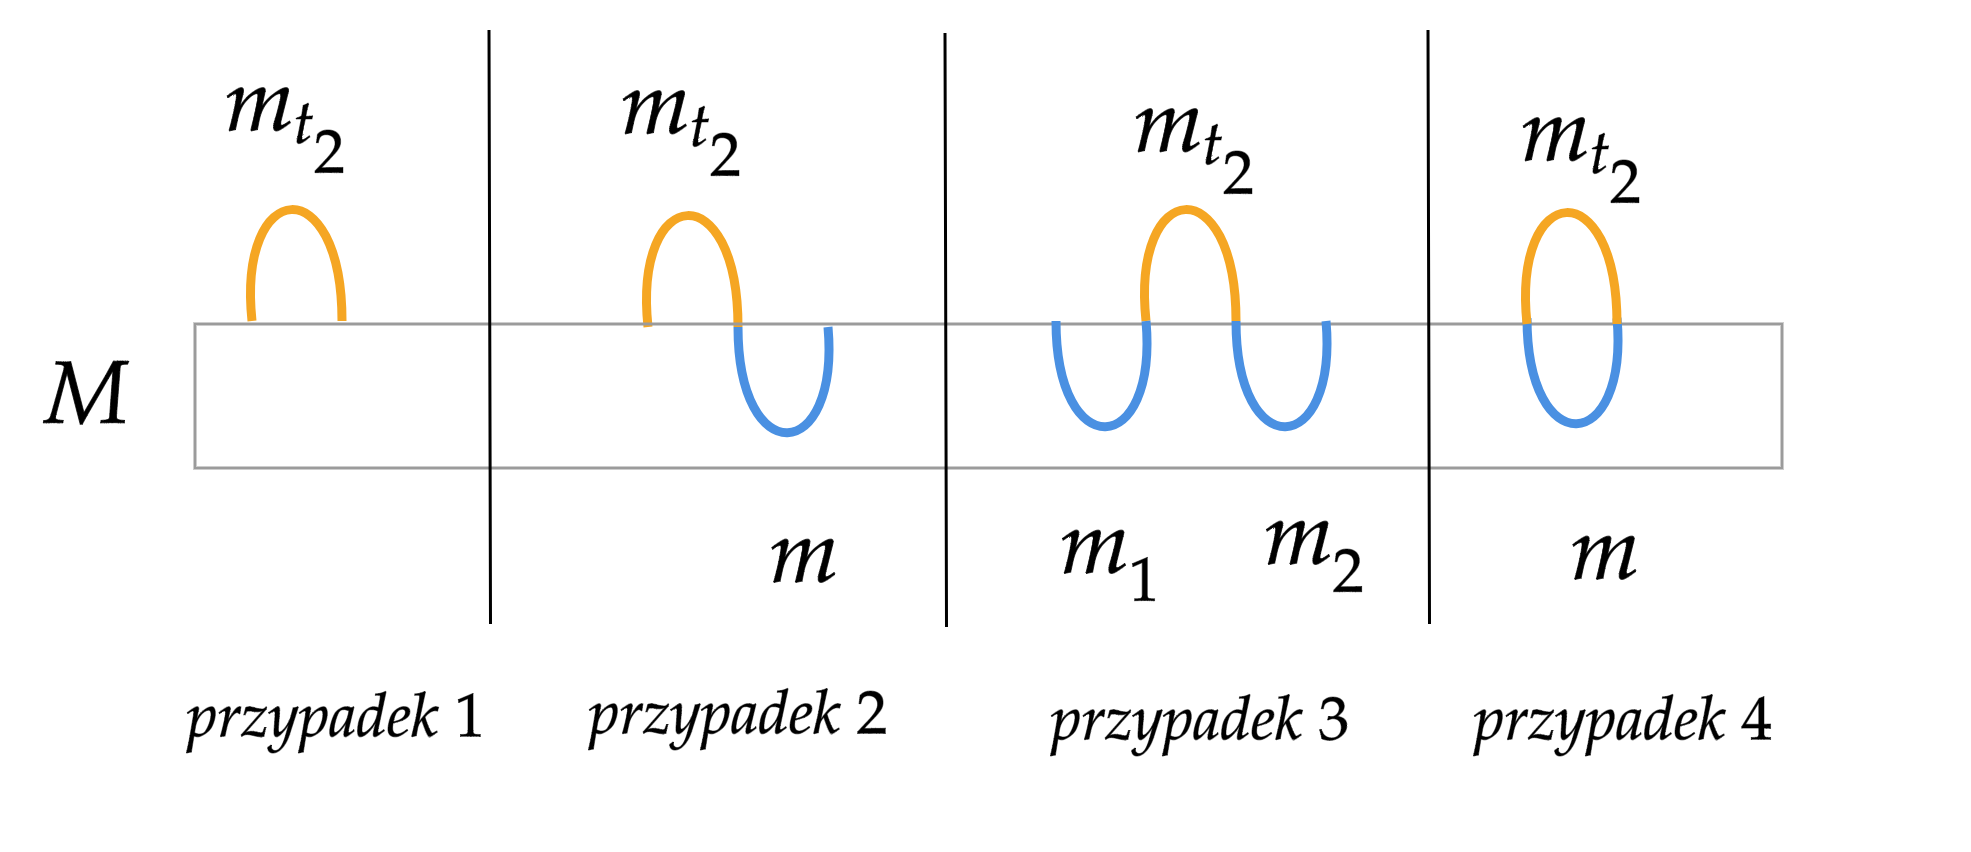
\includegraphics[width=16cm]{hamiltonian_merge2.png}
\caption{Dodawanie nowej krawędzi $m_{t_2}$ do skojarzenia $M$.}
\end{figure}

\texttt{SCALAJĄCY} - zauważmy, że scalane $F_{t_1}$ oraz $F_{t_2}$ nie mają wspólnych krawędzi, jedynie wierzchołki. Z powyższego wynika, że dla każdego wierzchołka $u$ należącego do $X_t$: $deg_t(u) = deg_{t_1}(u) + deg_{t_2}(u)$. Zauważmy, że musi być spełniony warunek $deg_t(u) \leq 2$. Jeśli $\mathcal{D}_{t_1}$ i $\mathcal{D}_{t_2}$ nie spełniają tego warunku, nie rozpatrujemy ich. Jednakże nie jest to warunek wystarczający, by rozwiązanie częściowe w kubełku $t$ było poprawne. Może się zdarzyć (jak przy dodawaniu krawędzi), że scalanie utworzy nam cykl. Scalając $M_{t_1}$ i $M_{t_2}$ uzupełniamy nasze obecne $M$ najpierw skojarzonymi wierzchołkami $m_{t_1} \in M_{t_1}$, by następnie pojednczo dodawać $m_{t_2} \in M_{t_2}$. Dla każdego nowo dodawanego $m_{t_2} = \{u, w\}$, sprawdzamy wszystkie $m \in M$, rozważając następujące przypadki (zobrazowane na rys. \ref{hamiltonian_merge}):
\begin{enumerate}
\item $\forall_{m \in M}: m_{t_2} \cap m = \emptyset$, do skojarzenia $M$ dorzucamy $m_{t_2}$.
\item $\exists_{m = \{v, z\} \in M}: \abs{m_{t_2} \cap m} = 1 \wedge \forall_{m^{\prime} \in M, m^{\prime} \ne m}: m_{t_2} \cap m^{\prime} = \emptyset$ - bez straty ogólności załóżmy, że $u = v$, czyli $m_{t_2} \cap m = \{u\}$, z $M$ usuwamy $m$ i dorzucamy nowe skojarzenie $\{w, z\}$.
\item $\exists_{m_1 = \{v_1, z_1\} \in M}: \abs{m_{t_2} \cap m_1} = 1 \wedge \exists_{m_2 = \{v_2, z_2\} \in M, m_2 \ne m_1}: \abs{m_{t_2} \cap m_2} = 1$ - bez straty ogólności załóżmy, że $u = v_1$ i $w = v_2$ (istotnym spostrzeżeniem jest fakt, że $m_{t_2} \cap m_1 \ne m_{t_2} \cap m_2$), usuwamy $m_1$ i $m_2$ z $M$ oraz dodajemy nowe skojarzenie $\{z_1, z_2\}$.
\item $\exists_{m \in M}: \abs{m_{t_2} \cap m} = 2$ - \texttt{CYKL}, $M_{t_1}$ i $M_{t_2}$ nie utworzą nam poprawnego rozwiązania.
\end{enumerate}

Końcowy wynik dla trójki $(t, \mathcal{D}, M)$ jest alternatywą po wszystkich $(t_1, \mathcal{D}_{t_1}, M_{t_1})$ i $(t_2, \mathcal{D}_{t_2}, M_{t_2})$, które spełniają wyżej wymienione warunki:

$$c[t][\mathcal{D}][M] = \bigvee \limits_{\mathcal{D}_{t_1}, \mathcal{D}_{t_2}, M_{t_1}, M_{t_2}} c[t_1][\mathcal{D}_{t_1}][M_{t_1}] \wedge c[t_2][\mathcal{D}_{t_2}][M_{t_2}]$$

Dla każdego kubełka mamy nie więcej niż $3^k \cdot k^k$ stanów. Zatem złożoność czasowa standardowego algorytmu dynamicznego po dekompozycji drzewowej dla problemu istnienia cyklu Hamiltona wynosi $k^{\Omicron(k)} \cdot n$, gdzie $n$ jest liczbą wierzchołków grafu $G$ danego na wejściu. 

\newpage
  	\chapter{Algorytmy dynamiczne z zastosowaniem techniki Cut \& Count}

W poprzednim rozdziale zostały przedstawione klasyczne algorytmy dynamiczne po dekompozycji drzewowej dla dwóch problemów decyzyjnych: drzewa Steinera oraz cyklu Hamiltona. Złożoność czasowa obu tych algorytmów jest niesatysfakcjonująca, gdyż zależy od $k^{\Omicron{(k)}}$ (gdzie $k$ jest szerokością drzewową). Czynnik ten jest następtwem trzymania odpowiednio: wszystkich możliwych podziałów cząstkowego drzewa Steinera na spójne poddrzewa oraz wszystkich możliwych skojarzeń wierzchołków wiszących w pary reprezentujące ścieżki będące częścią szukanego cyklu Hamiltona. W tym rodziale przedstawię dynamiczne algorytmy randomizowane (po dekompozycji drzewowej), bazujące na technice Cut \& Count opublikowanej przez ..., która znosi konieczność śledzenia podziału na partycje czy skojarzenia, tym samym znacznie poprawiając złożoność czasową w stosunku do klasycznych algorytmów dynamicznych. Technika Cut \& Count redukuje problemy decyzyjne do problemów zliczania wszystkich możliwych rozwiązań modulo $2$, jednocześnie dopuszczając rozwiązania niespójne (las w przypadku drzewa Steinera, zbiór cykli w przypadku cyklu Hamiltona). Technika Cut \& Count bazuje na tymczasowym poluzowywaniu ograniczeń dotyczących spójności szukanych rozwiązań, z tego względu znajduje ona uniwersalne zastosowanie tylko do problemów o spójnych rozwiązaniach.

    	\section{Drzewo Steinera}
Podobnie jak w poprzednim rozdziale, mamy dany graf $G$ wraz ze zbiorem terminali $K \subseteq V(G)$ oraz jego dekompozycję drzewową $\mathcal{T} = (T, \{X_t\}_{t \in V(T)})$. Dodatkowo dostajemy liczbę naturalną $\ell$. Pytamy, czy istnieje drzewo Steinera o rozmiarze co najwyżej $\ell$, innymi słowy: czy istnieje spójny graf acykliczny łączący wszystkie terminale, o co najwyżej $\ell$ krawędziach.


\newpage
	\begin{thebibliography}{9}
		\bibitem{kloks} 
			T. Kloks. 
			\textit{Treewidth. Computations and approximations}. 
			Lecture Notes in Computer Science, 842, 1994.
 
		\bibitem{bodlaender} 
			H. L. Bodlaender. 
			\textit{A linear-time algorithm for finding tree-decompositions of small treewidth}. 
			SIAM J. Comput. 25:6 (1996) 1305-1317
			
		\bibitem{robertson&seymour} 
			N. Robertson and P. D. Seymour. 
			\textit{Graph Minors II. Algorithmic aspects of treewidth}. 
			J. Algorithms 7 (1986) 309-322
 
		\bibitem{knuthwebsite} 
			Knuth: Computers and Typesetting,
			\\\texttt{http://www-cs-faculty.stanford.edu/\~{}uno/abcde.html}
	\end{thebibliography} 



\end{document}
